% TCC — Controle Adaptativo de Taxa de Bits para Jogos em Nuvem (Sunshine)
% Autor: César Morais — UFMG, 2026
% Compilação: pdflatex main && bibtex main && pdflatex main && pdflatex main

\documentclass[conference]{IEEEtran}

% ─── Encoding / Idioma ──────────────────────────────────────────────
\usepackage[utf8]{inputenc}
\usepackage[T1]{fontenc}
\usepackage[brazil]{babel}

% ─── Matemática / Tabelas / Figuras ─────────────────────────────────
\usepackage{amsmath,amssymb}
\usepackage{graphicx}
\usepackage{booktabs}
\usepackage{multirow}
\usepackage{array}
\usepackage{siunitx}

% ─── Código / Listings ──────────────────────────────────────────────
\usepackage{listings}
\usepackage{xcolor}
\lstset{
  basicstyle=\ttfamily\footnotesize,
  breaklines=true,
  showstringspaces=false,
  frame=single,
  language=C++
}

% ─── Hyperref por último ────────────────────────────────────────────
\usepackage[hidelinks]{hyperref}
\usepackage{cleveref}

% ─── Convenções ─────────────────────────────────────────────────────
\newcommand{\rtt}{RTT}
\newcommand{\kbps}{kbps}

\begin{document}

\title{Controle Adaptativo de Taxa de Bits para Jogos em Nuvem:\\
Uma Contribuição ao Servidor de Streaming Sunshine}

\author{\IEEEauthorblockN{César Pereira Morais}
\IEEEauthorblockA{Departamento de Ciência da Computação\\
Universidade Federal de Minas Gerais (UFMG)\\
Belo Horizonte, Brasil\\
cesarcreeper@gmail.com}}

\maketitle

\begin{abstract}
% TODO: 150–200 palavras. Problema, abordagem, resultado principal (queda
% de até 43\% no pico de RTT vs. AIMD de base), contribuição (código
% aberto incorporado ao Sunshine).
\end{abstract}

\begin{IEEEkeywords}
jogos em nuvem, controle de congestionamento, taxa de bits adaptativa,
AIMD, CUBIC, Sunshine, streaming de jogos.
\end{IEEEkeywords}

\section{Introdução}\label{sec:introducao}

% ─── Beat 1: O problema. ─────────────────────────────────────────────
% Jogos em nuvem: cliente fino, servidor caro, rede no meio.
% Requisitos duros: RTT < 100 ms, perda < 1\%.
% A rede doméstica não os respeita o tempo todo.

% ─── Beat 2: Por que controle adaptativo de taxa de bits importa. ────
% Sem ABR: estouro de buffer (bufferbloat), travamentos, recuperação
% via I-frame (IDR) — punição visual severa.
% O servidor é o lugar natural para o controle: ele controla o codec.

% ─── Beat 3: O Sunshine e o problema das plataformas comerciais. ────
% Plataformas comerciais (GeForce NOW, Xbox Cloud Gaming, PlayStation
% Plus) resolvem o problema às custas de lock-in: assinatura mensal,
% catálogo restrito, hardware proprietário no data center, sem controle
% do usuário sobre qualidade/latência. Alternativa open-source: o
% \emph{Sunshine}, servidor de streaming compatível com o protocolo
% NVIDIA GameStream (cliente Moonlight), permite que o usuário rode o
% próprio jogo na própria máquina e estreame para qualquer dispositivo
% leve em sua rede ou via internet. Hoje, opera com taxa de bits fixa
% negociada no início da sessão — sem reação a degradação de rede em
% curso, deixando a experiência refém da estabilidade do link.

% ─── Beat 4: A contribuição. ────────────────────────────────────────
% Implementamos um controlador AIMD com primitivas do CUBIC
% (Ha, Rhee, Xu, 2008) — curva cúbica de recuperação e convergência
% rápida — apenas com sinais observáveis no servidor (RTT, sem
% cooperação do cliente). Avaliamos contra (a) base sem ABR e
% (b) AIMD de duas fases sob seis cenários de degradação reproduzíveis.

% ─── Beat 5: Resultado principal. ───────────────────────────────────
% Redução de até 43\% no pico de RTT e até 60\% no tempo total de
% travamento, ao custo de um leve aumento na latência mediana — uma
% troca alinhada às prioridades de jogabilidade discutidas em
% \cite{alos2019,abragame}.

% ─── Beat 6: Estrutura do trabalho. ─────────────────────────────────
\subsection{Estrutura do Trabalho}
% Cap. \ref{sec:referencial} apresenta o referencial teórico e os
% trabalhos correlatos. Cap. \ref{sec:contribuicao} descreve o
% controlador proposto. Cap. \ref{sec:metodologia} detalha o testbed
% e o protocolo experimental. Cap. \ref{sec:resultados} apresenta os
% resultados. Cap. \ref{sec:conclusao} conclui e aponta trabalhos
% futuros.


\section{Referencial Teórico}\label{sec:referencial}

Esta seção apresenta uma revisão sistemática da literatura
relevante para controle adaptativo de taxa de bits em jogos em
nuvem. A revisão foi estruturada em seis eixos temáticos
complementares, conduzidos do mais geral ao mais específico:
caracterização do problema de rede em jogos em nuvem, codecs de
vídeo e reconfiguração em tempo de execução, controle de
congestionamento na herança do TCP, controle adaptativo para
mídia em tempo real, o trabalho mais próximo da contribuição
proposta, e o servidor \emph{Sunshine} como plataforma de
contribuição.

\subsection{Jogos em Nuvem como Problema de Rede}

Jogos em nuvem (\emph{cloud gaming}) consistem em executar o
jogo em um servidor remoto, capturar a saída de vídeo do jogo,
codificá-la em tempo real e transmiti-la a um cliente leve, que
decodifica e exibe os quadros enquanto envia comandos de entrada
de volta ao servidor. A arquitetura delega ao
servidor a carga computacional (GPU, codec), reduzindo o cliente
a um decodificador de vídeo — viabilizando jogos de alto custo
em hardware modesto.

Esta separação, no entanto, impõe requisitos rigorosos ao canal de rede. A revisão sistemática conduzida por Baldovino~\cite{baldovino2022}, abrangendo 33 estudos publicados entre 2017 e 2022, consolida os limiares tradicionalmente adotados pela literatura para caracterizar as condições necessárias à operação adequada de sistemas de cloud gaming: latência de ida e volta inferior
a \SI{100}{\milli\second} para jogos de ação, taxa de perda
inferior a 1\%, e tempo de resposta total (\emph{response time})
entre 100 e \SI{150}{\milli\second}. Acima desses limiares, a
experiência do usuário degrada de forma perceptível e, em casos
extremos, torna o jogo injogável.

A importância desses limiares está associada a uma característica fundamental do próprio meio. Diferentemente do \emph{streaming} de vídeo sob demanda, em que \emph{buffers} de alguns segundos conseguem mascarar variações da rede de forma praticamente transparente ao usuário, aplicações de cloud gaming operam com \emph{buffers} reduzidos, geralmente limitados a um ou dois quadros, para manter a interatividade. Como consequência, atrasos, perdas de pacotes ou variações na latência (\emph{jitter}) são rapidamente refletidos na qualidade percebida, manifestando-se na forma de travamentos, \emph{tearing} ou perda de sincronização.

Hong et al.~\cite{hong2015} avaliaram três jogos executados a 720p sobre o \emph{GamingAnywhere} e observaram que o MOS (\emph{Mean Opinion Score}) tende a saturar em torno de \SI{2}{\mega\bit\per\second}. Acima desse valor, aumentos na taxa de bits produzem ganhos perceptuais limitados; abaixo dele, a qualidade percebida se deteriora rapidamente. Esse comportamento reforça a importância de considerar métricas de cauda, como valores de pico e percentis elevados (p99), em vez de medidas centrais como a mediana, abordagem que será retomada no Capítulo~\ref{sec:metodologia}.

Como o processo de codificação é executado no servidor, este possui controle direto sobre a principal variável reconfigurável do pipeline: a taxa de bits-alvo do codificador. O servidor constitui, portanto, o ponto mais natural para a implementação da política de adaptação, dispensando mecanismos adicionais de cooperação por parte do cliente ou da infraestrutura de rede. Essa observação motiva o recorte adotado neste trabalho, detalhado no Capítulo~\ref{sec:contribuicao}.


\subsection{Codecs de Vídeo e Reconfiguração em Tempo de Execução}

A compressão de vídeo em jogos em nuvem é dominada pelos padrões
H.264, HEVC (H.265) e, mais recentemente, AV1, todos baseados em
predição temporal entre quadros. Três tipos de quadros compõem
um fluxo típico: quadros-I (\emph{intra-coded}), codificados de
forma independente; quadros-P (\emph{predicted}), que dependem
de quadros anteriores; e quadros-B (\emph{bidirectional}),
ausentes em jogos em nuvem por exigirem buffer adiante. Dentro
da categoria de quadros-I, os quadros IDR (\emph{Instantaneous
Decoder Refresh}) zeram a referência do decodificador, isolando
o erro de propagação após perdas — funcionando como mecanismo de
recuperação de último recurso quando outras escadas de proteção
(FEC, retransmissão seletiva) falham.

Entretanto, o custo dos quadros IDR é alto: por carregarem todo o
conteúdo do quadro de forma independente, IDRs são
substancialmente maiores que quadros-P, gerando picos abruptos
no tráfego de saída. Quando o canal já se encontra próximo da
saturação, a inserção de um IDR pode provocar enfileiramento no
gargalo, elevando o RTT (\emph{round-trip time}) e desencadeando
uma cascata: o cliente, ao não receber o IDR a tempo, solicita
outro, perpetuando o ciclo. Reduzir a frequência de IDRs é,
portanto, um objetivo indireto, mas relevante, do controle
adaptativo de taxa de bits.

A reconfiguração dinâmica da taxa de bits do codificador é
suportada pelos principais \emph{encoders} de hardware modernos. O trabalho de Hong et al.~\cite{hong2015}
foi pioneiro em estender o servidor open-source
\emph{GamingAnywhere} (GA) — antecessor direto do Sunshine — com
suporte a reconfiguração de codec em tempo de execução, antes
indisponível na plataforma. O presente trabalho herda
diretamente esta linha: opera sobre uma plataforma open-source
sucessora do GA e contribui exatamente com a política de decisão
que aciona essa reconfiguração — não com a reconfiguração em si,
que o Sunshine já suporta.

\subsection{Controle de Congestionamento: do TCP ao Streaming}

O controle de congestionamento na Internet é historicamente baseado no TCP. A família clássica de algoritmos TCP --- incluindo Reno, NewReno e SACK --- segue a política AIMD (\emph{Additive Increase, Multiplicative Decrease}), em que a janela de congestionamento cresce de forma aditiva na ausência de perdas e é reduzida multiplicativamente quando uma perda é detectada. Embora estável e amplamente estudada, essa estratégia apresenta limitações em redes com alto produto banda-atraso. Em um enlace de \SI{10}{\giga\bit\per\second} e RTT de \SI{100}{\milli\second}, por exemplo, o TCP clássico levaria aproximadamente 1,4 horas para recuperar a taxa de transmissão após uma única perda, o que o torna inadequado para diversas aplicações práticas~\cite{cubic}.

Para contornar essa limitação, Ha, Rhee e Xu propuseram o algoritmo CUBIC~\cite{cubic}, que substitui o crescimento linear da janela por uma função cúbica dependente do tempo transcorrido desde a última redução:
\begin{equation}
B(t) = C \cdot (t - K)^3 + W_{\max}
\label{eq:cubic}
\end{equation}

onde $W_{\max}$ representa o tamanho da janela imediatamente antes da última perda, $K$ corresponde ao instante em que a curva retorna a esse valor, e $C$ é uma constante que determina a taxa de crescimento. Para $t < K$, a curva é côncava e promove uma recuperação rápida em direção ao valor anteriormente alcançado. Nas proximidades de $t = K$, o crescimento torna-se mais gradual, enquanto para $t > K$ a curva assume formato convexo e passa a explorar capacidades adicionais da rede. Dessa forma, o CUBIC combina recuperação rápida após perdas com uma expansão mais cuidadosa acima do último ponto de operação conhecido.

CUBIC introduz adicionalmente o mecanismo de \emph{fast
convergence} (Equação 3.7 do trabalho original), que reduz
$W_{\max}$ quando uma nova redução é disparada antes da
recuperação completa. O efeito é prático: em cenários de
congestionamento sustentado, em que a capacidade real do
caminho está abaixo do último $W_{\max}$ conhecido, o algoritmo
deixa de mirar um teto obsoleto, convergindo para a capacidade
efetiva.

CUBIC é o algoritmo de controle de congestionamento \emph{default}
no kernel Linux desde a versão 2.6.18 (2006) e também o
mais implantado na Internet. Sua relevância para este trabalho é dupla. Em primeiro lugar,
o CUBIC fornece uma estratégia de recuperação amplamente estudada
na literatura, capaz de substituir a heurística de crescimento
utilizada pelo controlador de referência previamente avaliado.
Além disso, o mecanismo de \emph{fast convergence} contribui para
evitar a persistência de valores máximos incompatíveis com a
capacidade efetiva do caminho em situações de congestionamento
prolongado. A adaptação desses mecanismos ao contexto de mídia em
tempo real é apresentada no Capítulo~\ref{sec:contribuicao}.

\subsection{Controle Adaptativo para Mídia em Tempo Real}

O controle de congestionamento em fluxos de mídia em tempo real
sobre UDP — em que retransmissão é inviável e o sinal de perda
chega tardio — exige sinais distintos do TCP. Dois trabalhos
estabelecem o estado da arte fora do contexto específico de
jogos em nuvem.

\subsubsection{GCC --- Google Congestion Control}

O algoritmo GCC, descrito por Carlucci et al.~\cite{gcc}, é o controlador de congestionamento utilizado pelo WebRTC e incorporado em aplicações como Chromium e Google Hangouts. Diferentemente do TCP clássico, o GCC não utiliza a perda de pacotes como principal sinal de congestionamento. Em vez disso, baseia-se na variação do atraso unidirecional entre pacotes consecutivos para detectar o início da formação de filas, ajustando a taxa de envio por meio de uma política AIMD. Essa abordagem prioriza a manutenção de baixa latência em detrimento da máxima utilização da largura de banda, característica desejável em aplicações sensíveis a atraso, como videoconferência e cloud gaming.

O GCC reforça algumas das premissas adotadas neste trabalho. Em primeiro lugar, indica que, em aplicações de mídia em tempo real, sinais baseados em atraso tendem a ser mais adequados do que sinais baseados em perda. Além disso, mostra que estratégias inspiradas em AIMD continuam sendo eficazes quando adaptadas às características da aplicação. Por fim, demonstra que o controle pode ser implementado inteiramente do lado do remetente, exigindo apenas os mecanismos de \emph{feedback} já disponíveis. No WebRTC, esse papel é desempenhado pelo RTCP; no Sunshine, utiliza-se o RTT mantido pela biblioteca ENet no canal de controle do protocolo Moonlight.

A principal diferença em relação à abordagem proposta está na granularidade do controle. Enquanto o GCC opera em nível de pacote e recebe \emph{feedback} contínuo do receptor, o controlador desenvolvido neste trabalho atua em nível de quadro e utiliza amostras de RTT obtidas a cada ciclo de decisão. Essa escolha decorre das características do protocolo de streaming empregado e do custo associado a modificações no protocolo Moonlight.

\subsubsection{ABRAGame}

O algoritmo ABRAGame, proposto por Armendariz e
Joskowicz~\cite{abragame}, representa o trabalho mais recente em
controle adaptativo de taxa de bits especificamente voltado a
jogos em nuvem. O sinal central é \emph{latência cumulativa em
uma janela deslizante de \SI{500}{\milli\second}}, calculado no
cliente a partir de medições de atraso unidirecional amostradas
a cada \SI{20}{\milli\second}. A política prioriza
explicitamente \emph{estabilidade sobre qualidade}: aceita
reduções agressivas de resolução em troca de evitar travamentos
e quadros congelados, alinhando-se à assimetria de QoE
identificada por Hong et al.~\cite{hong2015}.

ABRAGame reforça a importância de métricas baseadas em atraso em aplicações de cloud gaming e a prioridade atribuída à estabilidade percebida pelo usuário. A principal diferença em relação à abordagem proposta neste trabalho está no requisito de sincronização entre os relógios do cliente e do servidor. O cálculo do atraso unidirecional pressupõe que ambos estejam sincronizados, condição difícil de garantir em redes domésticas e indisponível no protocolo Moonlight sem modificações adicionais. Em contraste, nossa abordagem opera exclusivamente sobre RTT, métrica mantida pela biblioteca ENet no canal de controle e já exposta pelo Sunshine, dispensando qualquer cooperação adicional do cliente.

\subsection{O Trabalho Mais Próximo: C\textsuperscript{3}G}

Dentre os trabalhos relacionados, o mais próximo da abordagem proposta é o C\textsuperscript{3}G (\emph{Congestion Control for Cloud Gaming over UDP based on Round-Trip Video Latency}), de Alós et al.~\cite{alos2019}. O C\textsuperscript{3}G é um controlador de taxa de bits do lado servidor, baseado em latência e inspirado em conceitos do algoritmo BBR (\emph{Bottleneck Bandwidth and RTT}), tendo sido implementado sobre a plataforma de cloud gaming PlayGiga.

Seu sinal principal, denominado \emph{Round-Trip Video Latency} (RTVL), corresponde a uma estimativa, calculada por quadro, do tempo transcorrido entre o início da codificação no servidor e a chegada da confirmação correspondente do cliente. A partir dessa métrica, o controlador combina uma fase reativa, responsável por reduzir a taxa de bits quando o RTVL excede determinados limiares, com uma fase proativa, em que informações de estados previamente observados orientam novas sondagens de taxa.

Embora compartilhe com o C\textsuperscript{3}G a utilização de sinais de atraso para controle adaptativo no servidor, a abordagem proposta neste trabalho difere em alguns aspectos importantes. Enquanto o C\textsuperscript{3}G depende do envio de confirmações associadas a cada quadro de vídeo, exigindo modificações no protocolo de \emph{streaming}, nossa implementação utiliza apenas o RTT já mantido pela biblioteca ENet no canal de controle do Moonlight. Além disso, a proposta é incorporada ao Sunshine, um projeto open-source amplamente utilizado pela comunidade de cloud gaming self-hosted, em contraste com a plataforma proprietária PlayGiga utilizada pelos autores.

Outra diferença está no mecanismo de recuperação após reduções de taxa. Em vez da heurística baseada em um dicionário de estados empregada pelo C\textsuperscript{3}G, adotamos a curva de crescimento do algoritmo CUBIC~\cite{cubic}, amplamente estudada na literatura de controle de congestionamento. Por fim, o compromisso entre utilização do canal e picos de atraso discutido por Alós et al. é mantido como referência para a avaliação experimental, permitindo comparar os resultados obtidos com aqueles reportados pelo estado da arte.

\subsection{O Servidor Sunshine}

O \emph{Sunshine} é um servidor open-source de \emph{streaming}
de jogos compatível com o protocolo NVIDIA GameStream e cliente
Moonlight, mantido sob a licença GPL-3.0 pela comunidade
LizardByte. Surgiu como uma alternativa open-source mais recente ao GamingAnywhere — plataforma alvo do trabalho de Hong et al.~\cite{hong2015} —, oferecendo suporte oferecendo suporte multiplataforma e múltiplos mecanismos de captura e codificação de vídeo.
Sua posição como alternativa \emph{self-hosted} a plataformas
comerciais como GeForce NOW e Xbox Cloud Gaming torna-o um
veículo de impacto direto para contribuições em jogos em nuvem.

O pipeline interno do Sunshine encadeia captura de tela,
codificação, encapsulamento e envio sobre UDP — vídeo com
proteção Reed-Solomon (FEC) e canal de controle sobre ENet —,
com a taxa de bits do codificador negociada uma única vez ao
início da sessão por meio do protocolo RTSP. Após a negociação
inicial, o servidor opera com taxa de bits fixa: não há, na
linha base, qualquer mecanismo de reação a degradação observada
do canal. Essa limitação motiva a proposta apresentada neste trabalho.

O Capítulo~\ref{sec:contribuicao} descreve a política de controle
proposta e sua integração na arquitetura do Sunshine; o
Capítulo~\ref{sec:metodologia} detalha o protocolo experimental
de avaliação.


\section{Contribuição}\label{sec:contribuicao}

Este capítulo apresenta o \emph{AIMD CUBIC}, controlador
adaptativo de taxa de bits proposto para o Sunshine. A
exposição segue cinco eixos: o recorte do problema e as
decisões de projeto que o delimitam; a visão geral da política
de controle; o detalhamento do algoritmo de detecção e atuação;
a justificativa para a cadência de decisão e o uso de
histerese; e, por fim, a descrição da integração do controlador
na arquitetura do Sunshine.

\subsection{Recorte do Problema}

A política de controle proposta foi delimitada por três decisões de projeto que precedem qualquer escolha algorítmica. A primeira estabelece que toda a lógica opera no servidor, utilizando apenas sinais já disponíveis no Sunshine, sem modificações no protocolo Moonlight nem cooperação adicional do cliente. Essa restrição é motivada por questões práticas: o Sunshine compartilha o protocolo com clientes Moonlight de terceiros, cuja evolução está fora do controle do projeto, tornando inviável qualquer requisito de extensão. A segunda decisão é a adoção do RTT como sinal único, em contraposição a métricas que exigiriam sincronização de relógio ou \emph{feedback} adicional por quadro. O RTT é mantido continuamente pela biblioteca ENet no canal de controle e já é exposto pelo Sunshine, o que o torna o sinal de menor custo operacional disponível.

A terceira decisão consiste em priorizar métricas de cauda da distribuição de latência, como picos, p99 e eventos de \emph{stall}, em detrimento de medidas centrais como a mediana (p50). Essa escolha decorre da assimetria de QoE discutida no Capítulo~\ref{sec:referencial}: ganhos acima do patamar de saturação do MOS são marginais, enquanto degradações abaixo dele comprometem significativamente a jogabilidade.

Esse recorte diferencia diretamente o presente trabalho do
estado da arte mais próximo. O C\textsuperscript{3}G de Alós et
al.~\cite{alos2019} também opera no servidor, mas depende do
envio de confirmação por quadro de vídeo, exigindo extensão do
protocolo. O ABRAGame de Armendariz e
Joskowicz~\cite{abragame} opera majoritariamente no cliente e
pressupõe sincronização de relógio para o cálculo de atraso
unidirecional. O GCC de Carlucci et al.~\cite{gcc} opera por
pacote sobre \emph{feedback} RTCP contínuo, granularidade
incompatível com o canal de controle do Moonlight. Cada uma
dessas abordagens é viável em seu ambiente original; nenhuma é
diretamente transplantável ao Sunshine sem custos arquiteturais
substanciais.

\subsection{Visão Geral do Controlador}

O \emph{AIMD CUBIC} é uma política de controle baseada em \emph{Additive Increase, Multiplicative Decrease} (AIMD), complementada por dois mecanismos do algoritmo CUBIC~\cite{cubic}: a curva cúbica de recuperação após reduções de taxa e o mecanismo de \emph{fast convergence} para atualização do teto de referência. O controlador é organizado como uma máquina de estados composta por cinco estados (estável, congestionado, decrescendo, recuperando e sondando), sendo avaliado periodicamente a partir de amostras de RTT obtidas durante a transmissão.

As amostras de RTT são coletadas continuamente ao longo da transmissão e utilizadas para atualizar os contadores de duração contínua acima e abaixo dos limiares configurados. As decisões de controle, entretanto, são tomadas em uma cadência fixa de 1~Hz, desacoplada da taxa de quadros do codificador. Em cada ciclo de decisão, o controlador determina se a taxa de bits-alvo deve ser mantida, reduzida ou aumentada. Reduções são disparadas quando o RTT permanece acima do limiar por um intervalo correspondente à histerese configurada, enquanto aumentos ocorrem após períodos sustentados abaixo do limiar e seguem a curva cúbica do CUBIC para definir a magnitude do incremento.


\begin{figure}[!t]
  \centering
  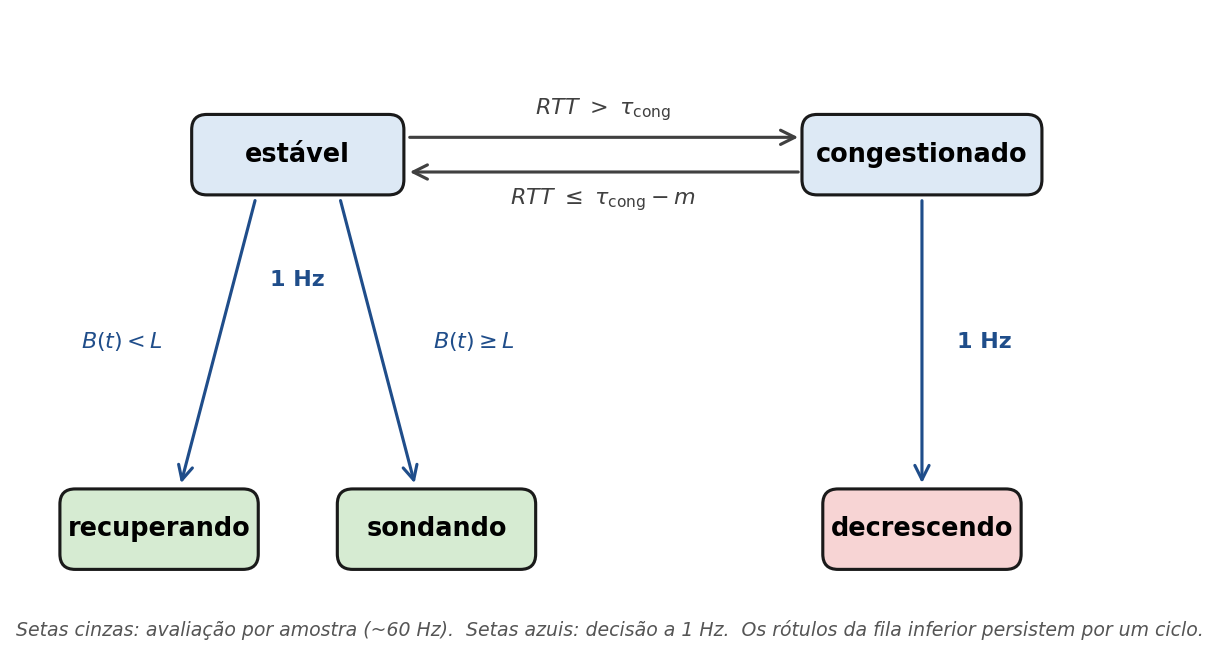
\includegraphics[width=\columnwidth]{images/state_machine.png}
  \caption{Máquina de estados do controlador AIMD CUBIC. A
  cada amostra de RTT (setas cinzas), o controlador transita
  entre os estados \emph{estável} e \emph{congestionado}
  conforme o RTT ultrapassa o limiar $\tau_{\rm cong}$ ou
  retorna abaixo de $\tau_{\rm cong} - m$, onde $m$ é a margem
  de histerese. A cada ciclo de decisão a 1~Hz (setas azuis),
  e desde que o \emph{streak} de duração mínima associado
  ($h_{\rm down}$ para decrementos, $h_{\rm up}$ para
  incrementos) tenha sido acumulado, o controlador atua sobre
  a taxa de bits-alvo do codificador: \emph{decrescendo} a
  partir de \emph{congestionado}; \emph{recuperando} ou
  \emph{sondando} a partir de \emph{estável}, conforme a
  amostra $B(t)$ da curva cúbica de recuperação esteja abaixo
  ou acima do teto $L$. Os rótulos da fila inferior persistem
  até o próximo ciclo de decisão.}
  \label{fig:state-machine}
\end{figure}

\subsection{Algoritmo}

\subsubsection{Sinal e Detecção}

O controlador recebe, a cada quadro codificado, uma amostra de
RTT proveniente da biblioteca ENet. A partir dessa amostra, dois
contadores de duração são mantidos. O primeiro, denominado
\emph{streak} de congestão, registra o início da janela contínua
mais recente em que o RTT permanece acima do limiar de
referência $\tau_{\text{cong}}$; é reiniciado sempre que uma
amostra retorna a valores aceitáveis. O segundo, denominado
\emph{streak} de via livre, registra simetricamente o início da
janela contínua em que o RTT permanece abaixo de
$\tau_{\text{cong}} - m$, onde $m$ é uma margem de histerese
introduzida pela razão discutida adiante. Os dois contadores são
atualizados continuamente, mas não disparam decisões por si só.

\subsubsection{Decremento Multiplicativo com \emph{Fast Convergence}}

Quando o \emph{streak} de congestão atinge uma duração mínima
$h_{\text{down}}$, o controlador aplica uma redução
multiplicativa à taxa atual:
\begin{equation}
  \text{kbps}_{\text{novo}} \gets \max\!\left( \beta \cdot \text{kbps}, \text{kbps}_{\min} \right)
  \label{eq:decrease}
\end{equation}
onde $\beta \in (0,1)$ é o fator de retenção e
$\text{kbps}_{\min}$ é o piso de operação. Empregamos $\beta = 0{,}7$,
valor utilizado no controlador AIMD de referência e mantido
nesta versão para isolar o efeito das demais alterações.

Antes da redução propriamente dita, o teto de recuperação
$L$ (último valor conhecido considerado seguro) é atualizado.
Em condições normais, em que a taxa atual ainda corresponde ao
último patamar estável, $L$ recebe o valor da taxa atual. Em
condições de congestionamento persistente, em que uma nova
redução é disparada antes que o controlador tenha recuperado o
patamar anterior, situação caracterizada por
$\text{kbps} < L$ no instante do disparo, $L$ é atualizado
segundo o mecanismo de fast convergence do
CUBIC:
\begin{equation}
  L \gets \text{kbps} \cdot \frac{1 + \beta}{2}
  \label{eq:fastconv}
\end{equation}
Esse ajuste retira do controlador a expectativa de retornar a
um teto que se mostrou inalcançável, fazendo-o convergir para
uma estimativa progressivamente mais próxima da capacidade
efetiva do canal. Em cenários de constrição prolongada, o
mecanismo evita que a curva de recuperação descrita a seguir
fique perpetuamente apontando para um valor obsoleto.

\subsubsection{Curva de Recuperação Cúbica}

Quando o \emph{streak} de via livre atinge uma duração mínima
$h_{\text{up}}$, o controlador aplica um incremento à taxa
atual. A magnitude do incremento é determinada por uma
amostragem da curva cúbica de recuperação do
CUBIC~\cite{cubic}:
\begin{equation}
  B(t) = C \cdot (t - K)^3 + L
  \label{eq:cubic-controller}
\end{equation}
onde $t$ é o tempo decorrido em segundos desde a última
redução, $L$ é o teto de recuperação definido por
(\ref{eq:fastconv}), $K$ é o tempo nominal de recuperação até
$L$, e $C = (1 - \beta) \cdot L / K^3$. A nova taxa-alvo é
$B(t)$, restrita ao intervalo $[\text{kbps},
\text{kbps}_{\max}]$, de modo que a curva nunca conduz a uma
redução, apenas a manutenção ou crescimento.

A forma de $B(t)$ é a mesma do CUBIC original, descrita no
Capítulo~\ref{sec:referencial}: côncava para $t < K$,
recuperando rapidamente em direção a $L$; aproximadamente
estável próximo de $t = K$; e convexa para $t > K$, sondando
de forma cautelosa, e depois acelerada, taxas acima do último
patamar conhecido. Para o presente trabalho, adotou-se
$K = 15$~s, valor calibrado empiricamente para que a fase de
sondagem inicie em uma escala compatível com a duração típica
de janelas de constrição nos cenários avaliados.

Variações na ancoragem temporal de $t$ e na regra de reinício do
\emph{streak} de via livre após crescimentos foram avaliadas
empiricamente, com resultados que motivam a forma adotada aqui;
essa análise é apresentada no
Capítulo~\ref{sec:resultados}, Seção~\ref{sec:sensibilidade}.

% [SUGESTÃO DE FIGURA] curva B(t) plotada para K=5s e K=15s
\begin{figure}[!t]
  \centering
  \includegraphics[width=\columnwidth]{figs/placeholder-cubic-curve}
  \caption{Curva de recuperação $B(t)$ amostrada pelo
  controlador AIMD CUBIC para dois valores do parâmetro $K$
  (\SI{5}{\second} e \SI{15}{\second}), com $\beta = 0{,}7$ e
  $L = 10\,000$~kbps. A região côncava ($t < K$) promove
  recuperação rápida em direção ao teto $L$; a região convexa
  ($t > K$) realiza sondagem cautelosa de capacidade adicional.}
  \label{fig:cubic-curve}
\end{figure}

\subsection{Cadência de Decisão e Histerese}

Duas decisões de projeto merecem justificativa explícita por
afetarem diretamente o comportamento dinâmico do controlador: a
cadência de avaliação a 1~Hz e o uso de histerese nos disparos
de decremento e incremento.

A cadência de 1~Hz é menor que a taxa de quadros do codificador
(tipicamente 60~Hz) por escolha deliberada. Reconfigurações
sucessivas e próximas no tempo da taxa do codificador
introduzem custos que vão da reinicialização de contextos
internos do \emph{encoder} ao envio de quadros IDR não
planejados, ambos potencialmente capazes de agravar a própria
condição de congestionamento que o controlador busca aliviar.
Espaçar as decisões em intervalos de um segundo permite que
cada atuação se propague pelo \emph{buffer} do gargalo e
manifeste seu efeito no RTT antes que a próxima decisão seja
tomada, evitando ciclos de realimentação curtos.

A histerese é um mecanismo clássico em sistemas de controle utilizado para evitar oscilações em torno de um limiar de decisão. No controlador proposto, ela é introduzida em dois níveis. Primeiro, exige-se que a condição de disparo (RTT sustentadamente acima ou abaixo do limiar) persista por uma duração mínima --- $h_{\text{down}}$ para decrementos e $h_{\text{up}}$ para incrementos --- antes que qualquer atuação ocorra. Esse requisito filtra picos transitórios de RTT, comuns em redes domésticas, que sob um critério instantâneo poderiam provocar uma sequência indesejada de cortes e recuperações.

Além disso, o controlador utiliza limiares distintos para identificar congestionamento e recuperação. Enquanto a entrada em congestionamento é caracterizada por RTT acima de $\tau_{\text{cong}}$, a condição de via livre exige que o RTT permaneça abaixo de $\tau_{\text{cong}}-m$, onde $m$ é uma margem de histerese. Dessa forma, pequenas oscilações do RTT em torno do limiar não fazem o controlador alternar continuamente entre os dois estados, permitindo que variações compatíveis com o ruído natural da rede sejam absorvidas sem disparar atuações desnecessárias.


Os valores adotados para todos os parâmetros do controlador são
sintetizados na Tabela~\ref{tab:params}. A escolha de cada
valor seguiu a calibração empírica conduzida ao longo do
desenvolvimento e descrita parcialmente no
Capítulo~\ref{sec:metodologia}.

\begin{table}[!t]
  \caption{Parâmetros do controlador AIMD CUBIC adotados na
  campanha experimental.}
  \label{tab:params}
  \centering
  \begin{tabular}{lll}
    \toprule
    \textbf{Parâmetro} & \textbf{Símbolo} & \textbf{Valor} \\
    \midrule
    Limiar de RTT (congestionamento) & $\tau_{\text{cong}}$ & \SI{100}{\milli\second} \\
    Margem de histerese & $m$ & \SI{20}{\milli\second} \\
    Histerese de decremento & $h_{\text{down}}$ & \SI{2000}{\milli\second} \\
    Histerese de incremento & $h_{\text{up}}$ & \SI{1000}{\milli\second} \\
    Fator de retenção & $\beta$ & 0{,}70 \\
    Tempo nominal de recuperação & $K$ & \SI{15}{\second} \\
    \emph{Fast convergence} & --- & ativo \\
    Intervalo de decisão & --- & \SI{1000}{\milli\second} \\
    Taxa mínima & $\text{kbps}_{\min}$ & \SI{1000}{\kilo\bit\per\second} \\
    Taxa máxima & $\text{kbps}_{\max}$ & inicial da sessão \\
    \bottomrule
  \end{tabular}
\end{table}

\subsection{Integração no Sunshine}

A política de controle foi implementada como uma classe
isolada em \texttt{src/bitrate\_controller.\{h,cpp\}}, contendo
exclusivamente lógica de decisão, sem qualquer acoplamento a
mecanismos de entrada ou saída do servidor. A classe expõe um
único método de atualização, \texttt{on\_sample}, que recebe
uma estrutura com a amostra de RTT corrente e retorna,
opcionalmente, uma nova taxa de bits-alvo quando uma decisão
de atuação é tomada. Essa separação preserva a testabilidade
do componente, viabilizando cobertura por testes unitários em
\emph{gtest} sob \texttt{tests/} sem necessidade de
infraestrutura de rede.

A integração com o restante do servidor ocorre em
\texttt{src/stream.cpp}, no laço principal de transmissão de
vídeo. A cada quadro codificado, a \emph{thread} de
\emph{broadcast} consulta o RTT corrente fornecido pela
biblioteca ENet e invoca \texttt{on\_sample}; quando o
controlador retorna uma nova taxa-alvo, a \emph{thread} aciona
o mecanismo de reconfiguração do codificador.

Os parâmetros do controlador foram expostos ao usuário em
\texttt{src/config.cpp}, junto aos demais parâmetros de
\emph{streaming}. A escolha de tornar os parâmetros
configuráveis, em vez de fixá-los no código, decorre da
expectativa de que diferentes perfis de uso, tipos de jogo e
condições típicas de rede do usuário possam exigir calibrações
próprias, e do reconhecimento de que a campanha
experimental conduzida neste trabalho cobre apenas um
subconjunto desses cenários. As mensagens visíveis ao usuário
adotam \texttt{boost::locale::translate} para internacionalização,
em conformidade com a convenção do projeto. O código segue as
diretrizes de formatação do \texttt{.clang-format} do
repositório e foi submetido como contribuição ao projeto
\emph{upstream}.

\section{Metodologia}\label{sec:metodologia}

Este capítulo descreve o ambiente experimental, o procedimento
de avaliação e os instrumentos utilizados para comparar o
controlador AIMD CUBIC com duas referências de base. A
organização segue seis eixos: o testbed físico e a carga de
trabalho adotada; os cenários de degradação de rede; os
controladores comparados; a instrumentação e as métricas
analisadas; o uso de inteligência artificial como ferramenta de
pesquisa; e o protocolo de execução das sessões experimentais.

\subsection{Testbed e Carga de Trabalho}

O servidor de \emph{streaming} executa o Sunshine sobre o
hardware descrito na Tabela~\ref{tab:testbed}. A escolha do
ambiente buscou aproximar-se de uma instalação típica de jogos
em nuvem \emph{self-hosted}: GPU dedicada da geração atual,
codificador NVENC, sistema operacional Linux, e conexão
cabeada ao roteador doméstico.

\begin{table}[!t]
  \caption{Especificações do testbed experimental.}
  \label{tab:testbed}
  \centering
  \begin{tabular}{ll}
    \toprule
    \textbf{Componente} & \textbf{Especificação} \\
    \midrule
    CPU (servidor) & AMD Ryzen 7 7700 (8 núcleos, 16 \emph{threads}) \\
    RAM (servidor) & 32~GB \\
    GPU (servidor) & NVIDIA GeForce RTX 4070 SUPER \\
    Codificador & NVENC \\
    Sistema operacional & Fedora Linux 43 \\
    \emph{Kernel} & Linux 6.19 \\
    Interface de rede (servidor) & Ethernet 1~Gbps \\
    Cliente & Smartphone Android, \emph{Moonlight} \\
    Conexão do cliente & Wi-Fi, mesma rede local \\
    \bottomrule
  \end{tabular}
\end{table}

A degradação de rede foi emulada no servidor via \texttt{tc}
com disciplina HTB, aplicada à interface de saída \texttt{eno1}.
Essa abordagem permite limitar a capacidade do enlace de forma
determinística e reproduzível, sem introduzir atrasos
artificiais que poderiam confundir o sinal de RTT utilizado
pelo controlador. Os \emph{scripts} de \emph{shaping} adotados estão disponíveis
no repositório do projeto.

A carga de trabalho utilizada em todas as sessões foi o jogo
\emph{Celeste}, escolhido por três motivos complementares. O
primeiro é o perfil de \emph{rendering} leve: o estilo
visual 2D mantém a taxa de bits demandada pelo codificador em
patamares relativamente estáveis, evitando que a variação do
canal seja confundida com variação do conteúdo. O segundo é a
sensibilidade do \emph{gameplay} à latência: a mecânica
baseia-se em saltos de precisão e janelas curtas de reação,
condição em que travamentos e atrasos são imediatamente
perceptíveis ao operador. O terceiro é a previsibilidade do
comportamento entre sessões, característica desejável para que
diferenças observadas entre controladores possam ser atribuídas
ao próprio controlador, e não ao conteúdo exibido. A escolha de
um único título constitui uma limitação reconhecida na
discussão dos resultados (Capítulo~\ref{sec:resultados}).

\subsection{Cenários de Avaliação}

Foram definidos seis cenários de degradação de rede,
sintetizados na Tabela~\ref{tab:scenarios}, escolhidos para
cobrir as principais formas em que um canal doméstico pode
degradar ao longo de uma sessão de jogo. Os cenários variam em
três dimensões complementares: a forma da degradação (queda
abrupta, em degraus, em janelas alternadas, ou contínua); a
severidade da constrição (de \SI{16}{\mega\bit\per\second}
até \SI{4}{\mega\bit\per\second}); e a duração total do
período sob shaping (de janelas curtas de \SI{30}{\second} a
constrições contínuas de \SI{160}{\second}). Fora das janelas
indicadas, o enlace opera sem restrição imposta pelo
\texttt{tc}, ou seja, na capacidade nativa de \SI{1}{\giga\bit\per\second}.

\begin{table}[!t]
  \caption{Cenários de degradação de rede utilizados na campanha
  experimental. Fora das janelas indicadas, o canal opera sem
  restrição.}
  \label{tab:scenarios}
  \centering
  \begin{tabular}{cll}
    \toprule
    \textbf{Cenário} & \textbf{Capacidade} & \textbf{Janela de shaping} \\
    \midrule
    A & 8~Mbps & 80--160~s \\
    B & 16 / 12 / 8~Mbps & 60--90 / 90--120 / 120--160~s \\
    C & 14 / 10~Mbps & 40--120 / 120--200~s \\
    D & 10~Mbps & 30--60 / 90--120 / 150--180 / 210--240~s \\
    E & 4~Mbps & 40--200~s \\
    F & 6~Mbps & 0--160~s \\
    \bottomrule
  \end{tabular}
\end{table}

O cenário~A representa uma queda abrupta e prolongada,
testando a capacidade do controlador de reagir a um corte
único e sustentado. O cenário~B aplica degraus sucessivos de
severidade crescente, exigindo do controlador adaptações
encadeadas em curto intervalo. O cenário~C aplica dois
patamares mais longos, simulando uma transição entre regimes
de banda. O cenário~D alterna entre quatro janelas curtas de
constrição e períodos de recuperação, testando o
comportamento do controlador em ciclos de degradação e
restauração. Os cenários~E e~F representam constrições
contínuas, severa e moderada respectivamente, em que o
controlador deve estabilizar a operação dentro do envelope
imposto pela rede.

\subsection{Controladores Comparados}

Três controladores foram avaliados, identificados como
referência fixa, AIMD de base e AIMD CUBIC. O controlador de
referência fixa corresponde ao comportamento original do
Sunshine, em que a taxa de bits é negociada uma única vez ao
início da sessão e mantida constante até o fim. O controlador
AIMD de base aplica corte multiplicativo com fator $\beta = 0{,}7$
ao detectar congestionamento e cresce em duas fases
(``$\times \gamma$ depois $+\Delta$''), sem o mecanismo de
\emph{fast convergence}; corresponde à versão do controlador
adaptativo que antecedeu a contribuição apresentada neste
trabalho. O controlador AIMD CUBIC corresponde à contribuição
descrita no Capítulo~\ref{sec:contribuicao}, com os parâmetros
sintetizados na Tabela~\ref{tab:params}.

\subsection{Instrumentação e Métricas}

A coleta de dados em \emph{runtime} é realizada pelo próprio
Sunshine, por meio de extensão de instrumentação introduzida em
contribuição prévia ao projeto. A cada amostra de RTT recebida
da biblioteca ENet, um registro é exportado para um arquivo
CSV contendo o instante de amostragem, o RTT, a variância do
RTT, o tempo de envio do quadro mais recente, o tamanho do
quadro codificado, a taxa de bits-alvo corrente, o estado do
controlador e indicadores de eventos relevantes (envio de
quadro IDR, requisição de IDR pelo cliente). A taxa de
amostragem é a própria taxa de quadros do codificador,
tipicamente próxima de \SI{60}{\hertz}.

A partir do CSV de cada sessão são derivadas as métricas
agregadas reportadas no Capítulo~\ref{sec:resultados}. As
métricas de latência incluem o pico de RTT, os percentis 50,
95 e 99 da distribuição, e a fração do tempo total em que o
RTT excede o limiar de \SI{100}{\milli\second} estabelecido
como referência para jogos de ação~\cite{baldovino2022}. As
métricas de throughput incluem a taxa de bits média sustentada
durante a janela de shaping e o uso do canal, definido como a
razão entre essa média e a capacidade imposta pela emulação.
As métricas de continuidade incluem a contagem de \emph{stalls},
definidos como intervalos consecutivos superiores a
\SI{100}{\milli\second} sem entrega de quadros ao cliente, o
tempo total acumulado em \emph{stall}, e a contagem de quadros
IDR emitidos durante a sessão. Esta última é utilizada como
indicador indireto de recuperação após perdas que escaparam aos
mecanismos de FEC.

Adicionalmente, ao final de cada sessão o operador registrou
três avaliações subjetivas em escala de 1 a 5, em que 1
corresponde à melhor avaliação: \emph{latência percebida},
\emph{qualidade visual} e \emph{estabilidade}. A avaliação foi
conduzida por um único operador (o autor do trabalho), o que
constitui uma limitação reconhecida na discussão dos
resultados.

\subsection{Uso de Inteligência Artificial como Ferramenta de Pesquisa}

Ferramentas de inteligência artificial baseadas em modelos de
linguagem de grande porte foram empregadas em dois pontos do
trabalho. O primeiro foi o apoio à implementação em C++ do
controlador e de sua integração ao Sunshine, incluindo o
ajuste de testes em \emph{gtest} e a conformidade com as
convenções de estilo do projeto \emph{upstream}. Todo o código
produzido com esse apoio foi revisado, compilado e testado pelo
pesquisador antes de qualquer submissão ao repositório
\emph{upstream}, e nenhuma alteração foi incorporada sem
verificação.

O segundo foi a estruturação de uma base de conhecimento
local, em formato Markdown compatível com o \emph{Obsidian},
utilizada como apoio à navegação do material bibliográfico, da
documentação interna do Sunshine, e do registro das iterações
de \emph{design} do controlador. A base é composta por
análises individuais (de \emph{papers} lidos, de subsistemas
do Sunshine e de Linux, e de cada iteração de projeto), com
referências cruzadas via \emph{wikilinks} que permitem
visualização em grafo. A síntese inicial de cada arquivo foi
auxiliada por IA a partir da leitura primária do material pelo
pesquisador, com edições e validações subsequentes realizadas
manualmente.

O uso de IA neste trabalho restringiu-se ao apoio à
implementação de código e à estruturação da base de
conhecimento de pesquisa, ambos sob revisão e validação do
pesquisador. As decisões de projeto, a análise dos resultados
experimentais e as conclusões apresentadas são de autoria
própria.

\subsection{Protocolo de Execução}

A campanha experimental consistiu em uma execução por par
(controlador, cenário) para o controlador AIMD CUBIC,
totalizando seis execuções novas. As colunas correspondentes
ao controlador de referência fixa e ao AIMD de base foram
reaproveitadas de campanha anterior, conduzida sobre o mesmo
testbed e com a mesma configuração do servidor, em razão da
baixa variância observada entre execuções repetidas naquela
campanha. As implicações dessa escolha são discutidas no
Capítulo~\ref{sec:resultados}.

Cada execução seguiu o mesmo procedimento. O servidor foi
iniciado com a configuração apropriada ao controlador em
avaliação. O cliente conectou-se ao servidor e iniciou o jogo
\emph{Celeste}, com o operador conduzindo o personagem por uma
sequência de fases pré-determinada, de duração total de
aproximadamente quatro minutos, suficiente para cobrir a janela
de shaping mais períodos de aquecimento e encerramento. O \emph{shaping} foi acionado no instante zero
da contagem do cenário, com a duração definida na
Tabela~\ref{tab:scenarios}. Ao final da sessão, o operador
registrou as três avaliações subjetivas descritas na seção
anterior. O arquivo CSV resultante foi arquivado em
\texttt{testbed/results/cubic/} com identificador associado ao
cenário e ao instante de execução.

\section{Resultados}\label{sec:resultados}

% ─── Beat 1: Visão consolidada. ─────────────────────────────────────
\subsection{Visão Geral}
% Tabela 3-vias × 6 cenários × métricas principais.
% Headline: AIMD CUBIC ganha em pico de RTT em 5/6 cenários
% (maior ganho: -43\% em A) e em tempo total de stall em 5/6
% (maior ganho: 11 s → 4,3 s em E), mas eleva p50/p95 em todos
% e perde ratings subjetivos em 3/6.

% ─── Beat 2: Por cenário. ───────────────────────────────────────────
\subsection{Análise por Cenário}

\subsubsection{Cenário A — Queda Abrupta}
% Caso onde CUBIC mais brilha: -43\% no pico.

\subsubsection{Cenário B — Degradação em Degraus}

\subsubsection{Cenário C — Dois Patamares}

\subsubsection{Cenário D — Janelas Curtas}

\subsubsection{Cenário E — Constrição Pesada Longa}
% Headline secundário: stalls 11 s → 4,3 s.

\subsubsection{Cenário F — Regressão Discutida}
% Único cenário em que CUBIC regride. Discutir por quê.

% ─── Beat 3: Trade-off central. ─────────────────────────────────────
\subsection{O Trade-off: Cauda vs. Regime Estacionário}
% CUBIC otimiza cauda da distribuição (pico, p99, stalls);
% AIMD de base otimiza regime estacionário (p50, p95).
% Esta é uma escolha de prioridade, não dominância.
% Conexão com \cite{alos2019} §6 (design philosophy).

% ─── Beat 3.5: Análise de sensibilidade ao design (5b/5c). ─────────
\subsection{Análise de Sensibilidade ao Design da Curva}\label{sec:sensibilidade}
% Após a comparação principal, avaliamos duas variantes de design da
% curva cúbica para entender o porquê da forma final adotada:
%
% - Variante 5b: âncora temporal em \texttt{rtt\_clear\_since} em vez
%   de \texttt{last\_decrease\_at}.
% - Variante 5c: acumulação monotônica de t entre crescimentos
%   (CUBIC literal, §3.1 do paper original).
%
% Ambas regridem o pico de RTT em cenários constrangidos (A K=5 s,
% E K=15 s). Diagnóstico estrutural: o CUBIC foi originalmente
% formulado para amostragem por-ACK, regime em que pequenos deltas
% acumulam ao longo de muitas iterações; em cadência de 1 Hz, a curva
% aplica o delta cheio em cada tick, resultando em overshoot
% sistemático.
%
% Achado de pesquisa a destacar: o CUBIC literal pressupõe densidade
% de amostragem por-ACK; em ambientes de cadência reduzida (1 Hz no
% nosso caso), a variante simplificada (âncora em last_decrease_at,
% reset de clear_since a cada crescimento) é não apenas suficiente,
% mas superior.
%
% Fontes: [[results-idea-5b]], [[results-idea-5c]].

% ─── Beat 4: Ratings subjetivos. ────────────────────────────────────
\subsection{Avaliação Subjetiva}
% Tabela de ratings 1-5 por cenário e controlador.
% n=1 avaliador. Limitação reconhecida.

% ─── Beat 5: Caveats. ───────────────────────────────────────────────
\subsection{Limitações dos Resultados}
% n=1 execução por célula CUBIC; reaproveitamento das colunas
% base; conteúdo do jogo afeta dificuldade efetiva (encoder produz
% menos quando cena é menos demandante); um único avaliador subjetivo.

\section{Conclusão}\label{sec:conclusao}

Este trabalho propôs e avaliou o \emph{AIMD CUBIC}, um
controlador adaptativo de taxa de bits para o servidor de
\emph{streaming} de jogos em nuvem Sunshine. O controlador
estende um esquema AIMD com duas primitivas do algoritmo
CUBIC~\cite{cubic}, a curva cúbica de recuperação após
reduções e o mecanismo de \emph{fast convergence}, e opera
exclusivamente a partir do RTT mantido pela biblioteca ENet
no canal de controle, sem qualquer cooperação adicional do
cliente. Avaliado contra um controlador de referência fixa e
uma variante AIMD de base ao longo de seis cenários de
degradação de rede, o controlador proposto reduz o pico de
RTT em cinco dos seis cenários, com a maior queda alcançando
43\% no cenário~A, e o tempo total acumulado em \emph{stall}
em cinco dos seis cenários, com queda de 61\% no cenário~E.
Esses ganhos são acompanhados de uma elevação sistemática do
RTT mediano, de 4--5~ms no AIMD de base para 12--23~ms no
AIMD CUBIC, configurando um trade-off explícito entre
desempenho na cauda da distribuição de latência e desempenho
no regime estacionário. Os dois controladores representam,
portanto, escolhas de prioridade complementares, não soluções
mutuamente dominantes.

\subsection{Achados que Transcendem o Sunshine}

A análise de sensibilidade ao design da curva (§\ref{sec:sensibilidade})
isolou um achado de alcance maior que a contribuição
imediata. Variantes mais fiéis à formulação original do CUBIC,
incluindo a interpretação literal do parágrafo §3.1 do
trabalho original, mostraram-se sistematicamente inferiores à
forma simplificada adotada neste trabalho. O diagnóstico é
estrutural: a curva cúbica do CUBIC foi formulada para
amostragem por~ACK, regime em que pequenos deltas se acumulam
ao longo de muitas iterações por segundo. Em controladores
amostrados a cadências reduzidas, como o aqui proposto em
1~Hz, a curva passa a aplicar o delta integral entre instantes
de decisão, e a fidelidade ao paper original deixa de ser
empiricamente desejável. A transposição de algoritmos de
controle de congestionamento entre regimes de cadência exige,
portanto, ajuste estrutural, não apenas reparametrização.

Dois outros achados merecem destaque. O primeiro é que o RTT
mantido server-side pela biblioteca ENet é, isoladamente,
sinal suficiente para um controlador útil em jogos em nuvem,
sem que sejam necessárias extensões de protocolo nem
sincronização de relógio entre cliente e servidor. O segundo é
que métricas de cauda (pico, percentil~99, eventos de
\emph{stall}) e métricas centrais (mediana, percentis
intermediários) devem ser reportadas conjuntamente para
caracterização correta de controladores adaptativos: nenhuma
das duas isoladamente é suficiente para distinguir prioridades
de projeto, e o desempenho subjetivo correlaciona de forma
não-trivial com ambas.

\subsection{Trabalhos Futuros}

Cinco direções concretas emergem como continuação natural
deste trabalho. A primeira é a introdução de uma memória de
capacidade efetiva entre sessões, motivada pela regressão
observada no cenário~F. Naquele cenário, a curva inicial de
recuperação fica apontada para o teto negociado de sessão,
inalcançável dada a constrição ativa desde $t=0$. Uma
estimativa de capacidade carregada da sessão anterior
permitiria que o controlador iniciasse com um teto
\texttt{last\_known\_good} mais próximo da capacidade real do
caminho, evitando a primeira cascata desperdiçada.

A segunda direção é a adoção de um sinal de detecção
sub-segundo, possivelmente a partir do tempo de envio do
quadro mais recente (\texttt{frame\_send\_ms}, já coletado na
instrumentação atual). A latência de reação do controlador
proposto é da ordem da histerese de decremento, e um sinal
adicional que se manifeste antes da inflação do RTT pode
encurtar o tempo entre o início do congestionamento e o corte
de taxa.

A terceira direção é a introdução de um gatilho preditivo
baseado em gradiente, na linha do controlador GCC para
WebRTC~\cite{gcc}, capaz de antecipar a transição da fase de
não-congestionamento para a fase de enfileiramento antes que
o RTT cruze o limiar.

A quarta direção é a condução de uma avaliação subjetiva
\emph{crowdsourced}, segundo o protocolo de Hong et
al.~\cite{hong2015}, em substituição às avaliações de
operador único conduzidas neste trabalho. Esse formato
permite quantificação estatística de Mean Opinion Score sob
diferentes perfis de jogador, tipos de jogo, e condições de
rede.

A quinta direção é a comparação direta do AIMD CUBIC contra o
GCC~\cite{gcc} e o ABRAGame~\cite{abragame} em um mesmo
testbed, com a mesma instrumentação. Embora os trabalhos
correlatos tenham reportado seu desempenho em ambientes
próprios, a comparação cruzada em ambiente comum é a única
forma robusta de posicionar o presente trabalho contra o
estado da arte em métricas absolutas.

\subsection{Impacto}

O controlador proposto, juntamente com a instrumentação de
coleta de métricas que o sustenta, será submetido como
contribuição ao repositório \emph{upstream} do Sunshine sob a
licença GPL-3.0 do projeto. O testbed experimental, os
\emph{scripts} de geração de cenários, os dados de cada
sessão e os \emph{notebooks} de análise estão disponíveis para
reprodução. As restrições metodológicas adotadas, como a
execução única por cenário, a padronização da carga de
trabalho em um único título e a avaliação subjetiva por um
único operador, são documentadas ao longo do trabalho e
abrem o caminho natural para as direções de trabalho futuro
listadas acima.


\bibliographystyle{IEEEtran}
\bibliography{bibliography}

\end{document}
